
\section{Bevezet\H o}
Inform\'aci\'o minden\"utt jelen van k\"or\"ul\"ott\"unk. A technol\'ogia fejl\H od\'es\'evel egyre t\"obbet \'es t\"obbet tudtunk bel\H ole digitaliz\'alni. Ez\'altal az adat rendelkez\'esre \'all, a k\'erd\'es az marad, hogy ezt hogyan tudjuk felhaszn\'alni.

Az ut\'obbi id\H oben jobban el\H ot\'erbe ker\"ult a vide\'ok\'arty\'ak nem csak j\'at\'ekokban val\'o kihaszn\'al\'asa, hanem nagym\'ert\'ekben t\"obbsz\'alas\'ithat\'o probl\'em\'ak nagy bemenetre val\'o felhaszn\'al\'asa.

Ugyanakkor a nagyobb sz\'am\'it\'asi kapacit\'as nem sokat \'er, ha a programoz\'o nem tudja kihaszn\'alni.
Vide\'ok\'arty\'ak \'altal\'anos c\'el\'u programoz\'asra a mostan\'aban jellemz\H o technol\'ogi\'ak a CUDA az NVIDIA-t\'ol illetve az OpenCL a Khronos Group-t\'ol. A CUDA nagyon gyors \'es el\'eg k\'enyelmes, a sok be\'ep\'itett funkci\'o j\'ovolt\'ab\'ol, amik nem csak levesznek a fejleszt\H o v\'all\'ar\'ol felel\H oss\'eget, de a v\'egletekig optimaliz\'alva van a hardverre. Cser\'ebe csak a gy\'art\'o vide\'ok\'arty\'ain t\'amogatott.
Az OpenCL egy ny\'ilt szabv\'any, \'es nem csak vide\'ok\'arty\'akon val\'o futtat\'ast t\'amogat, hanem egy\'eb hardvereszk\"oz\"oket is. Viszont a szabv\'any implement\'al\'asa a gy\'art\'ok feladata, amit p\'eld\'aul az NVIDIA nem siet el, \'igy a \H o k\'arty\'aikon nem olyan friss verzi\'ot t\'amogatnak. Ez mondjuk \'erthet\H o, hiszen nekik megvan a saj\'at eszk\"oz\"uk.
De ha a grafikus feladatokat n\'ezz\"uk az OpenGL egyre ink\'abb alulmaradt a DirectX-szel szemben, mind haszn\'alhat\'os\'ag, mint teljes\'itm\'eny szempontj\'ab\'ol.

Az OpenGL-\'ert felel\H os \href{https://www.khronos.org/}{Khronos Group} a 2015-\"os \href{http://www.gdconf.com/}{Game Developers Conference}-n bejelentette a Vulkan-t, mint egy alacsonyszint\H u, cross-platform sz\'am\'it\'asi \'es 3D grafika API.
2016 febru\'arj\'aban pedig kij\"ott az els\H o verzi\'o \'es az\'ota is t\"ort\'ennek fejleszt\'esek, illetve lassan, de egyre t\"obben mutatnak ir\'anta \'erdekl\H od\'est, k\"ozt\"uk p\'eld\'aul a nagyszab\'as\'u \href{https://robertsspaceindustries.com/star-citizen}{Star Citizen}.
%\footnote{\url{https://www.gamestar.hu/hir/star-citizen-directx-12-vulkan-api-226130.html}}

\subsection{Vulkan}
\begin{figure}[h]
	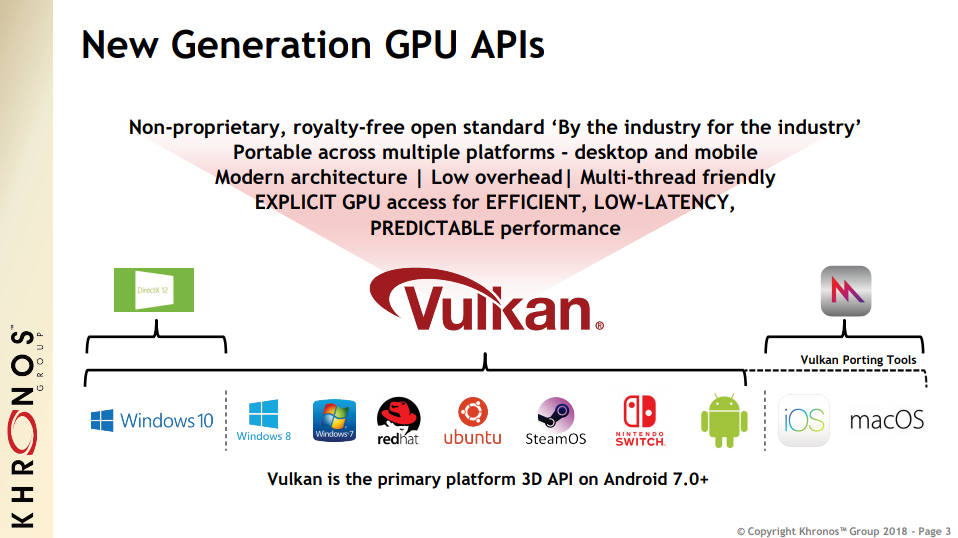
\includegraphics[width=\textwidth]{img/vulkanpromo}
	\centering
	\caption{Prom\'oci\'o az \'uj API-nak.
		\cite{vulkan1.1launchpres} }
\end{figure}
Maga az API az \href{https://www.amd.com/en-us/innovations/software-technologies/mantle}{AMD Mantle} egyfajta folytat\'asak\'ent is tekinthet\H o. Az elgondol\'as az, hogy pr\'ob\'aljunk min\'el jobb teljes\'itm\'enyt kinyerni a hardverb\H ol, CPU-GPU a terhel\'es jobb eloszt\'as\'aval.

A legjobb eredm\'enyhez az vezet, ha optimaliz\'aci\'os lehet\H os\'eget adunk azok kez\'ebe, akik jobban ismerik az adott alkalmaz\'ast: a fejleszt\H ok.
Ez\'altal nagyobb kontrollja van a fejleszt\H onek a program m\H uk\"od\'ese felett, a driverek is egyszer\H ubbek lesznek, ez\'altal a gy\'art\'ok elm\'eletben gyorsabban tudj\'ak az \'uj verzi\'okat t\'amogatni.

Cser\'ebe mivel t\"obb feladatk\"or h\'arul az alkalmaz\'as k\'esz\'it\H o(i)re, maga a fejleszt\'esi folyamat lehet hosszadalmasabb.

\subsection{Kiterjesztett val\'os\'ag}
AR alkalmaz\'asokban a megfelel\H o felhaszn\'al\'oi \'elm\'enyhez elengedhetetlen, hogy kis k\'es\'essel t\"ort\'enjen a felhaszn\'al\'o el\'e az inform\'aci\'o prezent\'al\'asa. 

Kicsit komolyabb p\'eld\'aval \'elve egy j\"ov\H obeli aut\'o AR sz\'elv\'ed\H oj\'en lehet a m\'asodperc t\"ored\'ek\'en m\'ulik egy \'elet, hogy megjelenjen valamilyen figyelmeztet\'es a s\"of\H ornek egy k\"ozelg\H o gyalogosr\'ol.

Tov\'abb\'a a Vulkan \'ig\'erete, hogy a driverek \'ir\'asa egyszer\H ubb lesz, \'igy ebben az esetben lehets\'eges az is, hogy az aut\'o be\'agyazott rendszer\'ere t\"ort\'en\H o fejleszt\'esi id\H o ler\"ovid\"ul, hiszen a fejleszt\H oknek nem kell valamilyen speci\'alisan arra a hardverre fejlesztett k\"ornyezettel megismerkedni\"uk. 

\subsection{Motiv\'aci\'o}

